% -- Anfang Präambel
\documentclass[german,  % Standardmäßig deutsche Eigenarten, englisch -> english
parskip=full,  % Absätze durch Leerzeile trennen
%bibliography=totoc,  % Literatur im Inhaltsverzeichnis (ist unüblich)
%draft,  % TODO: Entwurfsmodus -> entfernen für endgültige Version
]{scrartcl}
\usepackage[utf8]{inputenc}  % Kodierung der Datei
\usepackage[T1]{fontenc}  % Vollen Umfang der Schriftzeichen
\usepackage[ngerman]{babel}  % Sprache auf Deutsch (neue Rechtschreibung)

% Mathematik und Größen
\usepackage{amsmath}
\usepackage[locale=DE,  % deutsche Eigenarten, englisch -> US
separate-uncertainty,  % Unsicherheiten seperat angeben (mit ±)
]{siunitx}
\usepackage{physics}  % Erstellung von Gleichungen vereinfachen
\usepackage{yfonts}  % Frakturschrift für Real- und Imaginärteil komplexer Größen

\usepackage{graphicx}  % Bilder einbinden \includegraphics{Pfad/zur/Datei(ohne Dateiendung)}
\usepackage{svg}

% Gestaltung
%\usepackage{microtype}  % Mikrotypographie (kann man am Ende verwenden)
\usepackage{booktabs}  % schönere Tabellen
%\usepackage[toc]{multitoc}  % mehrspaltiges Inhaltsverzeichnis
\usepackage{csquotes}  % Anführungszeichen mit \enquote
\usepackage{caption}  % Anpassung der Bildunterschriften, Tabellenüberschriften
\usepackage{subcaption}  % Unterabbildungen, Untertabellen, …
\usepackage{enumitem}  % Listen anpassen
\setlist{itemsep=-10pt}  % Abstände zwischen Listenpunkten verringern

% Manipulation des Seitenstils
\usepackage{scrpage2}
% Kopf-/Fußzeilen setzen
\pagestyle{scrheadings}  % Stil für die Seite setzen
\clearscrheadings  % Stil zurücksetzen, um ihn neu zu definieren
\automark{section}  % Abschnittsnamen als Seitenbeschriftung verwenden
\ofoot{\pagemark}  % Seitenzahl außen in Fußzeile
\ihead{\headmark}  % Seitenbeschriftung mittig in Kopfzeile
\setheadsepline{.5pt}  % Kopzeile durch Linie abtrennen

\usepackage[hidelinks]{hyperref}  % Links und weitere PDF-Features

% TODO: Titel und Autor, … festlegen
\newcommand*{\titel}{Reaktor}
\newcommand*{\autor}{Tom Drechsler, Konstantin Schmid}
\newcommand*{\abk}{RE}
\newcommand*{\betreuer}{Dr. Carsten Lange}
\newcommand*{\messung}{28.02.2020}
\newcommand*{\ort}{AKR-2 (Pauer-Bau)}

\hypersetup{pdfauthor={\autor}, pdftitle={\titel}}  % PDF-Metadaten setzen

% automatischen Titel konfigurieren
\titlehead{Fortgeschrittenen-Praktikum \abk \hfill TU Dresden}
\subject{Versuchsprotokoll}
\title{\titel}
\author{\autor}
\date{\begin{tabular}{ll}
Protokoll: & \today\\
Messung: & \messung\\
Ort: & \ort\\
Betreuer: & \betreuer\end{tabular}}

% -- Ende Präambel

\begin{document}
\begin{titlepage}
\maketitle  % Titel setzen
\tableofcontents  % Inhaltsverzeichnis
\end{titlepage}

% Text Anfang
\section{Versuchsziel und Aufgabenstellung}
Der Versuch Reaktor ist in zwei Teilversuche unterteilt: der Reaktorstart und die Steuerstabkalibrierung.
\\\\
1. Reaktorstart
\begin{itemize}
\item Die Funktionskontrolle des Reaktors ist gemäß Prüfvorschrift durchzuführen und zu
protokollieren.
\item Der Reaktor ist durch Wiederholungsstart in Betrieb zu nehmen und bei der in der Betriebsanweisung (BA) genannten thermischen Leistung kritisch zu machen.
\item  Zur qualitativen Untersuchung des Verhaltens eines Nullleistungsreaktors sind Leistungsänderungen gemäß Anweisung des Versuchsleiters durchzuführen.
\item An ausgewählten Messpunkten im Kontrollbereich ist die Gamma-Dosisleistung in
Abhängigkeit von der thermischen Leistung des Reaktors zu bestimmen.
\item In Abhängigkeit von der thermischen Leistung des Reaktors ist die kritische Stabstellung
zu ermitteln und zu diskutieren.
\end{itemize}
2. Steuerstabkalibrierung
\begin{itemize}
\item  Ein Steuerstab des Reaktors AKR ist in Abhängigkeit von der Stabposition nach der Methode der stabilen Reaktorperiode zu kalibrieren. Aus den gemessenen Verdopplungszeiten der Reaktorleistung sind die zugehörigen stabilen
Perioden und damit die Reaktivitätsäquivalente nach der INHOUR-Gleichung zu berechnen.
\item In Abhängigkeit von der Stabposition sind die differentielle Steuerstabkennlinie und die integrale Steuerstabkennlinie grafisch darzustellen.
\item Unter Zuhilfenahme der Kennlinien für die anderen Steuerstäbe des AKR sind die Überschussreaktivität und
die Abschaltreaktivität bei partieller Abschaltung zu ermitteln.
\end{itemize}
Ziel des Versuches Reaktor ist das Kennenlernen des prinzipiellen Aufbaus eines thermischen Reaktors und seiner Hauptkomponenten. Außerdem ist die Kenntnis der Eigenschaften der Steuerungs- und Regeleinrichtungen wichtig für den sicheren Betrieb des Reaktors.

\section{Theoretische Grundlagen}
\subsection{Kernspaltung und U-235}
Die theoretische Grundlage zur Kernspaltung bietet eine Betrachtung der Bindungsenergie pro Nukleon für verschiedene Elemente. Diese ist in Abbildung 1 zu sehen.
\\
\begin{figure}[h!]\centering
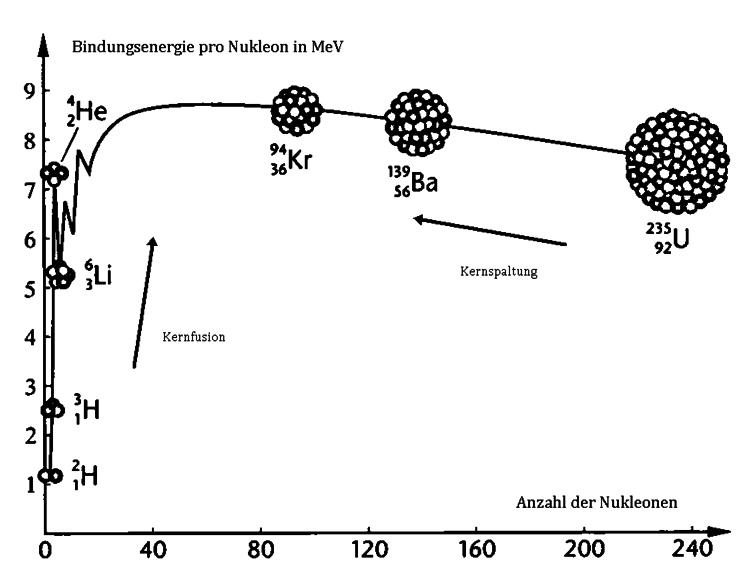
\includegraphics[width=0.8\textwidth]{bindungsenergie}
\caption{Mittlere Bindungsenergie pro Nukleon über der Nukleonenzahl, entnommen aus \cite{bindungsenergie}.}
\end{figure}
\\
Das Maximum der Bindungsenergie ist bei $^{56}_{26}$Fe erreicht, also bei einer Nukleonenzahl von $56$. Kerne von Elementen mit einer geringeren Nukleonenzahl als $56$, wie beispielsweise Wasserstoff, können fusioniert werden, sodass dabei deren Differenz der Bindungsenergie frei wird. Dies geschieht in Sternen wie unserer Sonne. Die Kernspaltung funktioniert genau andersherum. Kerne mit einer größeren Nukleonenzahl als $56$ werden gespalten, um deren Differenz der Bindungsenergie nutzen zu können.
\\\\
Im Fall des AKR-2 wird $^{235}_{92}$U verwendet. Dieses wird im Folgenden mit U-$235$ abgekürzt. Ein Urankern kann durch Neutronen gespalten werden. Allerdings eignen sich nicht alle Neutronen, um so eine Kernspaltung zu bewirken. Dies ist in Abbildung 2 zu erkennen.
\\\\
\begin{figure}[h!]\centering
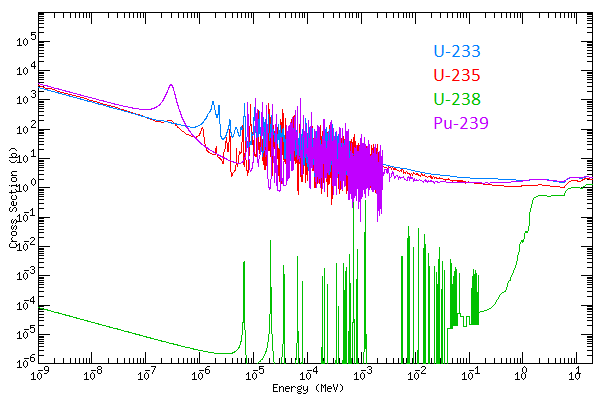
\includegraphics[width=0.8\textwidth]{sigma_neutronen}
\caption{Wirkungsquerschnitt von Neutronen über der Neutronenenergie für verschiedene Isotope von Uran und Pu-$239$, entnommen aus \cite{sigma_neutronen}.}
\end{figure}
\\
Für Neutronen mit geringer Energie ist der Wirkungsquerschnitt in der Größenordnung von $10^2$\,b bis $10^3$\,b. Für schnelle Neutronen hingegen ist der bis zu drei Größenordnungen geringer. Demzufolge sollten auch geringe Neutronenenergien verwendet werden. Diese langsameren Neutronen heißen thermische Neutronen und haben eine Energie von ca. $0.025$\,eV. Die Bezeichnung leitet sich aus einer Betrachtung der thermischen Energie ab:
\begin{align}
\langle E \rangle = \frac{3}{2} k_{\text{B}} T \approx  k_{\text{B}} T.
\end{align}
Bei Zimmertemperatur ergibt sich dies zu:
\begin{align}
\langle E \rangle \approx 0.025\,\text{eV}.
\end{align}
Die Neutronen befinden sich also bei dieser Energie im thermischen Gleichgewicht mit der Umgebung.
\\\\
Wenn ein Neutron nun auf einen Urankern trifft, erfolgt der Prozess, welcher in Abbildung 3 dargestellt ist.
\\\\\\\\\\
\begin{figure}[h!]\centering
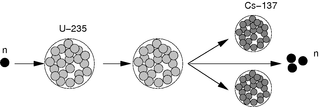
\includegraphics[width=0.8\textwidth]{spaltung_uran}
\caption{Schematische Darstellung der Spaltung von U-$235$, entnommen aus \cite{spaltung_uran}.}
\end{figure}
\\\\
Das Neutron trifft auf den Urankern und es entsteht ein instabiler Zwischenzustand der dann schließlich in zwei neue Kerne und Neutronen zerfällt. Die Zahl der entstehenden Neutronen ist zwei oder drei und abhängig von den Zerfallsprodukten. Die Zerfallsprodukte können sich in angeregten Zuständen befinden, sodass im Zuge des Reaktorbetriebes neben Neutronen auch $\gamma$-Strahlung entsteht. Im Mittel entstehen pro Spaltung ca. $2.47$ Neutronen. Diese haben allerdings eine höhere Energie, sodass diese abgebremst werden müssen, damit sie eine neue Spaltung in Gang bringen können. Dies geschieht durch einen sogenannten Moderator. Besonders gut eignen sich dafür Materialien, die Wasserstoffatome enthalten, denn die Masse eines Neutrons ist ähnlich groß wie die Masse eines Wasserstoffatoms beziehungsweise dessen Kern. Dies liefert nach der Impulsbilanz einen optimalen Energieverlust. Allerdings muss zudem eine weitere Charakteristik des Moderatormaterials berücksichtigt werden. Das Material darf die Neutronen nicht absorbieren. Deshalb wird zum Beispiel kein reiner Wasserstoff verwendet. Im Fall des AKR-2 wird ein Feststoff zur Moderation verwendet, nämlich Polyethylen, dessen chemische Struktur in Abbildung 4 dargestellt ist.
\\
\begin{figure}[h!]\centering
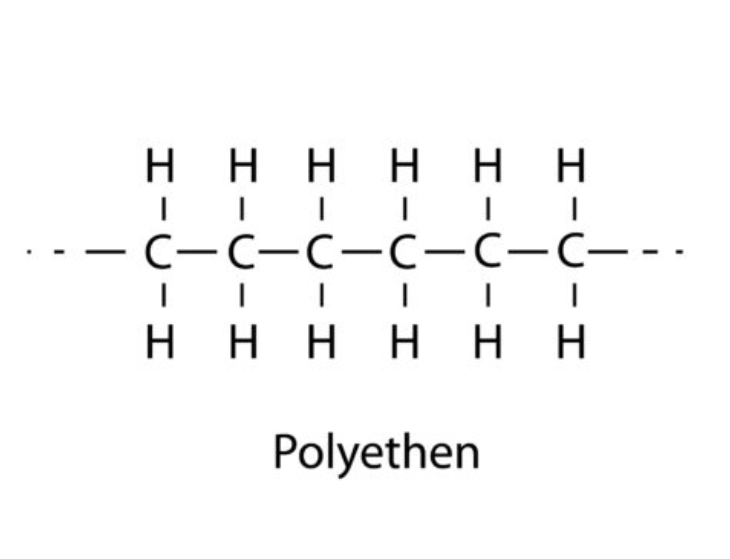
\includegraphics[width=0.55\textwidth]{pe}
\caption{Strukturformel für Polythylen, entnommen aus \cite{pe}.}
\end{figure}
\\
Die so abgebremsten thermischen Neutronen stehen zur Anregung neuer Spaltungen zur Verfügung. Auf diese Art und Weise entsteht eine Kettenreaktion, welche mit Hilfe der Steuerungseinrichtungen des Reaktors kontrolliert zur Energiegewinnung genutzt werden kann.

\subsection{Art des Reaktorstarts und Nullleistungsreaktor}
Es gibt verschiedene Arten des Reaktorstarts: das Anfahrexperiment, das kritische Experiment und den Wiederholungsstart. Im Rahmen dieses Versuchs wird ein Wiederholungsstart durchgeführt. Dieser ist dadurch charakterisiert, dass keine Änderungen an Einbauten und am Reaktor selbst vorgenommen wurden. Das Reaktivitätsverhalten unterscheidet sich also nicht zur letzten Inbetriebnahme. Somit sind bereits die kritischen Stellungen der Steuerstäbe bekannt. Zusammengefasst handelt es sich also um einen Anlassvorgang des routinemäßigen Reaktorbetriebes.
\\\\
Beim AKR-2 handelt es sich um einen Nullleistungsreaktor. Diese werden bei einer Leistung von wenigen Watt betrieben, sodass Effekte wie Brennstoffabbrand, Vergiftung des Brennstoffs und Temperatureffekte vernachlässigt werden können. Konkret für diesen Versuch wird maximal eine Leistung von $P = 2$\,W erreicht.

\subsection{Zustände des Reaktors}
Der jeweilige Zustand des Reaktors hinsichtlich der Neutronenproduktion wird mit dem Multiplikationsfaktor $k$ beschrieben. Dabei können drei Zustände unterschieden werden:
\begin{itemize}
\item unterkritisch: $k<1$ (Leistung $P$ des Reaktors sinkt)
\item kritisch: $k=1$ (Leistung $P$ des Reaktors bleibt konstant)
\item überkritisch: $k>1$ (Leistung $P$ des Reaktors steigt)
\end{itemize}
Daraus kann die Reaktivität $\rho$ definiert werden:
\begin{align}
\rho = \frac{k-1}{k}.
\end{align}
Diese kann noch auf einen Faktor $\beta$ normiert werden:
\begin{align}
\rho' = \frac{\rho}{\beta}.
\end{align}
Somit ergibt sich zur Charakterisierung des Reaktorzustandes eine Tabelle (siehe Abbildung 5).
\\
\begin{figure}[h!]\centering
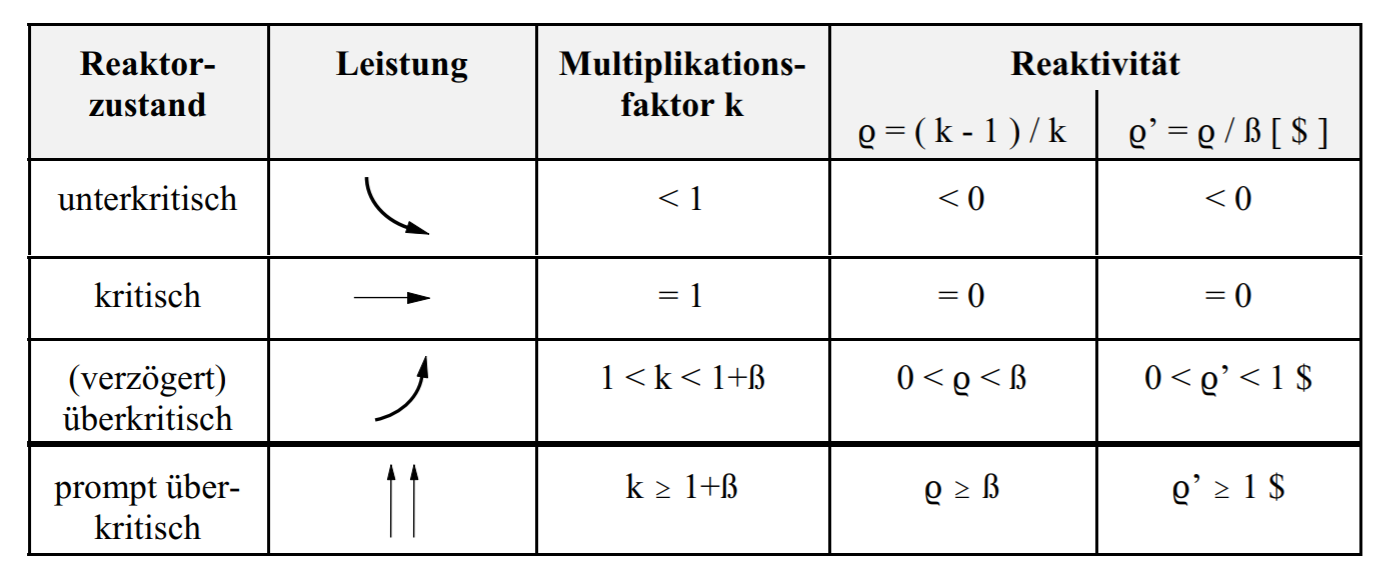
\includegraphics[width=0.8\textwidth]{zustand}
\caption{Tabelle der verschiedenen Reaktorzustände, entnommen aus \cite{1}.}
\end{figure}
\\
Die Bedeutung des Faktors $\beta$ wird im folgenden Abschnitt noch geklärt.
\\\\
Eine weitere wichtige Kenngröße des Reaktors ist die Reaktorperiode $T$. Sie ergibt sich als Parameter zur Beschreibung der Neutronenzahl nach Lösen der zugehörigen Differentialgleichung:
\begin{align}
N(t) = N(t=0) \cdot e^{\frac{t}{T}}.
\end{align}
$t$ beschreibt also, in welcher Zeit sich die Neutronenzahl um den Faktor $e$ ändert. Da dies allerdings eine schlechte Messgröße ist, wird die Verdopplungszeit $T_2$ eingeführt. Sie beschreibt, in welcher Zeit sich die Neutronenzahl verdoppelt. Es ergibt sich demzufolge dieser Zusammenhang:
\begin{align}
T_2 = \ln(2) \cdot T.
\end{align}

\subsection{Prompte und verzögerte Neutronen}
Die bei der Spaltung von Uran entstehenden Neutronen können in prompte und verzögerte Neutronen unterteilt werden. Prompte Neutronen entstehen unmittelbar bei der Kernspaltung, verzögerte Neutronen hingegen mit etwas Zeitversatz. Der Anteil verzögerter Neutronen wird dabei mit dem bereits verwendeten $\beta$ bezeichnet. Es gilt:
\begin{align}
\beta = 0.641\, \%.
\end{align}
Obwohl der Anteil $\beta$ also so gering ist, ermöglichen gerade diese verzögerten Neutronen die Steuerung eines solchen Reaktors.
\\\\
Die verzögerten Neutronen können nochmals in sechs Gruppen eingeteilt werden. Deren spezifische Eigenschaften sind in Abbildung 6 zusammengefasst.
\\
\begin{figure}[h!]\centering
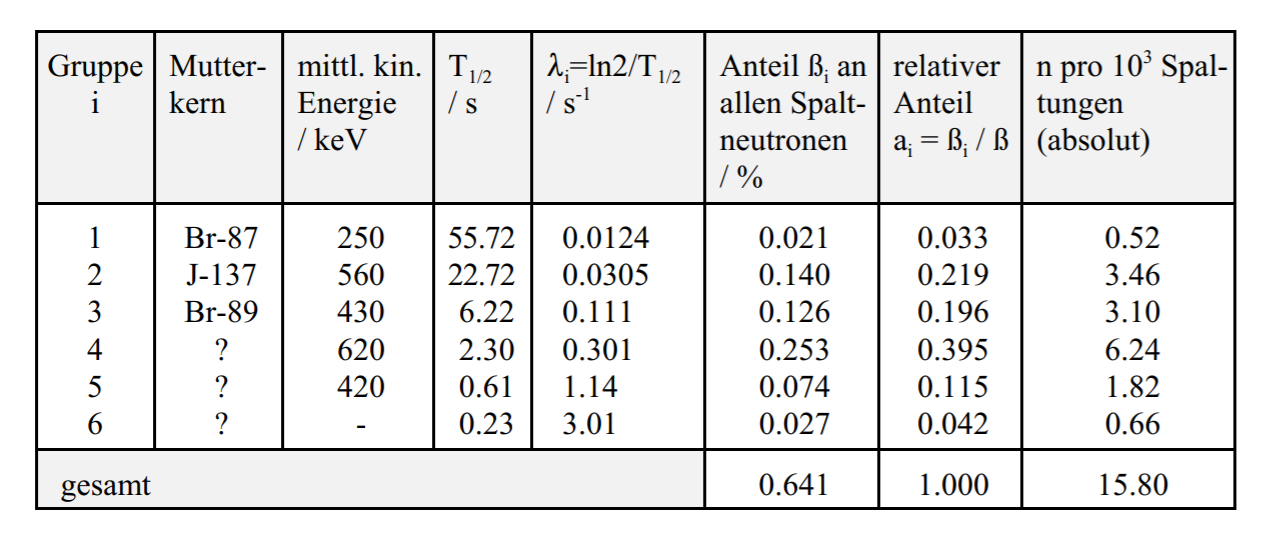
\includegraphics[width=0.8\textwidth]{eig}
\caption{Eigenschaften der verschiedenen Gruppen verzögerter Neutronen, entnommen aus \cite{1}.}
\end{figure}

\subsection{Aufbau und Funktionsweise des AKR-2}
Der schematische Aufbau des AKR-2 ist durch Abbildung 7 gegeben.
\\
\begin{figure}[h!]\centering
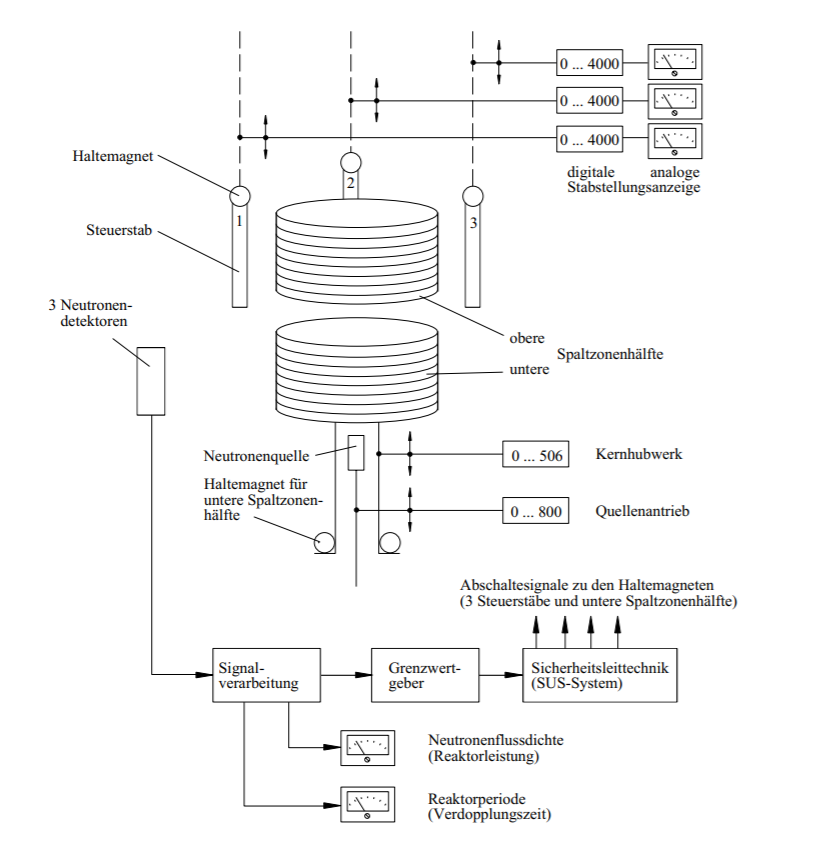
\includegraphics[width=0.7\textwidth]{aufbau}
\caption{Schematischer Aufbau des AKR-2, entnommen aus \cite{1}.}
\end{figure}
\\
Die zylindrische Spaltzone ist aus Sicherheitsgründen in zwei Hälften aufgeteilt. Darin befinden sich die Brennelemente, welche aus  zu $19.8\,\%$ angereichertem Uranoxid und dem Moderator Polyethylen bestehen. Um ein zu starkes Entweichen von Neutronen zu verhindern, ist die Spaltzone von einem Graphitreflektor umgeben. Eine Anfahrneutronenquelle (Am-Be-Quelle) wird zur Verringerung der statistischen Messunsicherheit verwendet. Da es sich bei den Neutronen um eine Zählstatistik handelt, kann eine Poissonverteilung angesetzt werden:
\begin{align}
\Delta N &= \sqrt{N} \\
\Rightarrow \frac{\Delta N}{N} &= \frac{1}{\sqrt{N}}.
\end{align}
Somit reduziert der Anfahrneutronenquelle die relative Messunsicherheit, sodass auch bei einer kleinen Neutronenzahl ein sinnvoll messbares Signal entsteht. Die drei Steuerstäbe des Reaktors bestehen aus Cadmium, die sowohl zur Steuerung als auch zur Sicherheitsabschaltung dienen.

\subsection{Steuerstabkennlinien}
Für die Steuerstäbe können die Reaktivitätskennwerte, die sogenannten Steuerstabkennlinien aufgenommen werden. Dabei wird jeweils auf der x-Achse die Eindringtiefe $z$ und auf der y-Achse jeweilig die differentielle Reaktivitätsänderung $\frac{d\rho}{dz}$ oder die integrale normierte Änderung $\frac{\rho}{\rho_{\text{max}}}$ dargestellt. Die so zu erwartenden Kurven haben den in Abbildung 8 dargestellten prinzipiellen Verlauf.
\\
\begin{figure}[h!]\centering
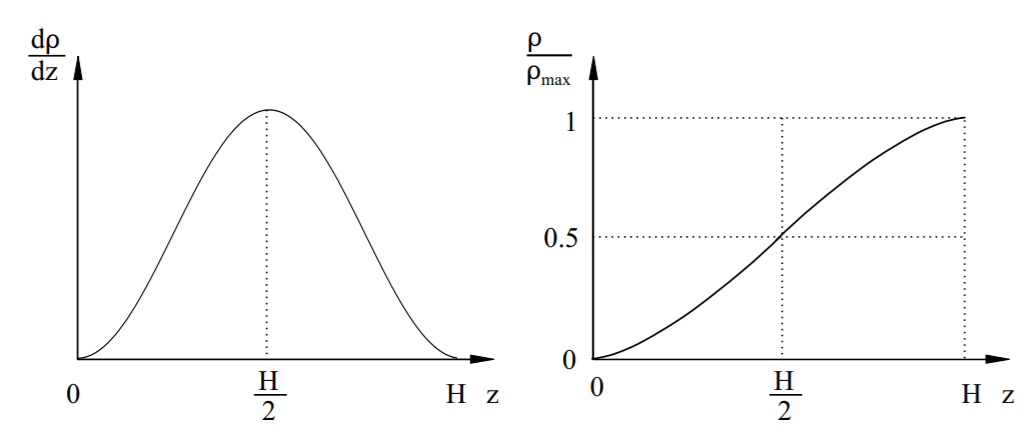
\includegraphics[width=0.9\textwidth]{kennlinien}
\caption{Qualitativer Verlauf der Steuerstabkennlinien. Differentiell links, integral rechts. Entnommen aus \cite{2}.}
\end{figure}
\\
Für die differentielle Kennlinie gilt:
\begin{align}
\Phi_z &= \Phi_z^{\text{max}} \cdot \sin\left(\frac{\pi \cdot z}{H} \right) \\
\Rightarrow \frac{d\rho}{dz} &= C \cdot \Sigma_a \cdot \Phi_z^2 \propto \sin^2\left(\frac{\pi \cdot z}{H} \right).
\end{align}
Für die integrale Kennlinie hingegen:
\begin{align}
\rho = \int_0^{z} \frac{d\rho}{dz} dz =  C \cdot \Sigma_a \cdot (\Phi_z^{\text{max}})^2 \cdot \frac{H}{\pi}
\left[\frac{\pi \cdot z}{2H} - \frac{1}{4} \ \sin\left(\frac{2\pi z}{H} \right) \right].
\end{align}
\subsection{Messung der stabilen Reaktorperiode und INHOUR-Gleichung}
Um die Reaktivitäten zu bestimmen, wird die Methode der Messung der stabilen Reaktorperiode verwendet. Theoretische Grundlage dafür sind die sogenannten reaktorkinetischen Grundgleichungen:
\begin{align}
\frac{dn}{dt} &= \frac{\rho - \beta}{l^*} \cdot n + \sum_{i=1}^{6}\lambda_i \cdot C_i + S \\
\frac{dC_i}{dt} &= \frac{\beta_i}{l^*} \cdot n - \lambda_i \cdot C_i.
\end{align}
Die darin auftretenden Größen sind:
\begin{itemize}
\item $l^*$ - mittlere Lebensdauer der prompten Neutronen
\item $\rho$ - Reaktivität
\item $\beta_i$ - absoluter Anteil der i-ten Gruppe verzögerter Neutronen
\item $C_i$ - Konzentration der Mutterkerne verzögerter Neutronen der i-ten Gruppe
\item $\lambda_i$ - Zerfallskonstante der Mutterkerne der i-ten Gruppe verzögerter Neutronen
\item $S$ - Neutronenquelle im Reaktor
\end{itemize}
Ansätze für die Lösung dieses Differentialgleichungssystems sind:
\begin{align}
n_i(t) &= n_i(t=0) \cdot e^{\omega_i \cdot t} \\
C_i(t) &= C_i(t=0) \cdot e^{\omega_i \cdot t}.
\end{align}
Die Gesamtlösung für $n(t)$ ist eine Superposition:
\begin{align}
n(t) = \sum_{i = 0}^{6} n_i(t) = \sum_{i = 0}^{6}  n_i(t=0) \cdot e^{\omega_i \cdot t}.
\end{align}
Allerdings ist bloß $\omega_{0}$ positiv, sodass die restlichen Terme exponentiell abklingen und nach einer kurzen Zeit nur noch Folgendes übrig bleibt:
\begin{align}
n(t) &= n_0(t=0) \cdot e^{\omega_0 \cdot t} \\
C(t) &= C_0(t=0) \cdot e^{\omega_0 \cdot t}.
\end{align}
Einsetzen in die reaktorkinetischen Grundgleichungen mit $\omega = \frac{1}{T}$ liefert die INHOUR-Gleichung:
\begin{align}
\rho = \frac{l^*}{T} + \sum_{i=1}^{6} \frac{\beta_i}{1+ \lambda_i \cdot T}.
\end{align}
Für kleine Reaktivitäten reduziert sich dies auf:
\begin{align}
\rho &\approx \frac{1}{T} \cdot \sum_{i=1}^{6} \frac{\beta_i}{\lambda_i}.
\end{align}
Für die normierte Reaktivität $\rho'$ gilt:
\begin{align}
\Rightarrow \rho' & = \frac{\rho}{\beta} \frac{l^* / \beta}{T} \cdot \sum_{i=1}^{6} \frac{a_i}{1+ \lambda_i \cdot T}.
\end{align}
Dabei ist $a_i = \frac{\beta_i}{\beta}$. Diese relativen Häufigkeiten können aus Abbildung 6 entnommen werden.
\section{Durchführung}
\subsection{Vorbereitung auf den Reaktorstart}
Nach einer Sicherheitsbelehrung, der Vorstellung des Reaktors sowie einer Besprechung grundlegender Verhaltensweisen und des Ablaufplans wurde der Reaktor gemäß den geltenden Vorschriften auf Funktionsfähigkeit überprüft und anschließend in Betrieb genommen. Um die gesetzlichen Bestimmungen des Strahlenschutzes zu gewährleisten, wurden zunächst folgende Schritte abgearbeitet:
\begin{enumerate}
\item Ausstattung aller Personen mit Schutzkitteln und tragbaren Dosimetern,
\item Kontrolle der Funktion des Hand-Fuß-Kleider-Monitors in der Personenschleuse durch die Betreuer,
\item Überprüfung des Vorhandenseins einer gültigen Betriebsanweisung,
\item Kontrolle des Vorhandenseins und der Funktionstüchtigeit des geeichten tragbaren, netz-unabhängigen Röntgen-Gamma-Dosimeters am Steuerpult des AKR,
\item Kontrolle des Vorhandenseins und der Funktionstüchtigeit des tragbaren, netzunabhängigen Neutronendosisleistungs-Messgerätes am Steuerpult des AKR und
\item Kontrolle der Betriebsbereitschaft der stationären Gamma-Ortsdosisleistungsmesskanäle in der Reaktorhalle (grünes Feld leuchtet).
\end{enumerate}
Auf diese Weise wird sichergestellt, dass vorgeschriebene Grenzwerte der Dosisleistung nicht überschritten werden, keine kontaminierten Personen oder Kleidungsstücke das Gebäude verlassen und neben den Messgeräten am Steuerpult weitere tragbare und vor allem unabhängige Messgeräte zur Verfügung stehen. \\\\
Für eine ordnungsgemäße Inbetriebnahme des Reaktors ist die Abschalteinrichtung auf Funktionsfähigkeit zu überprüfen, damit die Anlage falls nötig sicher abgeschaltet werden kann. Dazu werden folgende Schritte ausgeführt:
\begin{enumerate}
\item Zurücksetzen des RESA-Signals im Schutzsystem über einen Schlüsselschalter am Steuerpult zur Vorbereitung auf das Anfahren,
\item Einfahren der Neutronenquelle in die obere Endstellung,
\item Anheben der unteren Kernhälfte aus der unteren Endstellung
\item Abbruch des Hebevorgangs der unteren Kernhälfte, sobald das Verlassen der unteren Endstellung am Bildschirm sichtbar ist,
\item Manuelles Auslösen der Reaktorschnellabschaltung (im foilgenden RESA genannt) sowie
\item Kontrolle des Abfalls der unteren Spaltzonenhälfte; das erneute Erreichen der unteren Endlage muss angezeigt werden.
\end{enumerate} 
Durch diese Überprüfung ist sichergestellt, dass im Ernstfall jederzeit eine RESA ausgelöst werden kann und die dafür notwendigen technischen Mechanismen alle richtig funktionieren. Da es sich hier um einen Ausbildungsreaktor handelt, gibt es eine Anfahrverriegelung: Wird ein fest vorgeschriebenes Schema zum Anfahren des Reaktors nicht eingehalten oder werden während des Experiments bestimmte Grenzwerte der Leistung oder der Neutronenflussdichte nicht eingehalten, wird vom System automatisch eine RESA ausgelöst. Damit sollen Unfälle durch unsachgemäße Handhabung verhindert werden. Damit sind alle Überprüfungen abgeschlossen und der Reaktor kann gestartet werden. Der Vollständigkeit halber sei angemerkt, dass bei kritischen Experimenten noch weitere Überprüfungen nötig sind.
\subsection{Wiederholungsstart}
Der Wiederholungsstart hat nach einem vorgeschriebenen Ablaufplan zu erfolgen, welcher in Abb. 9 illustriert ist.
\newpage


\begin{figure}[h!]\centering
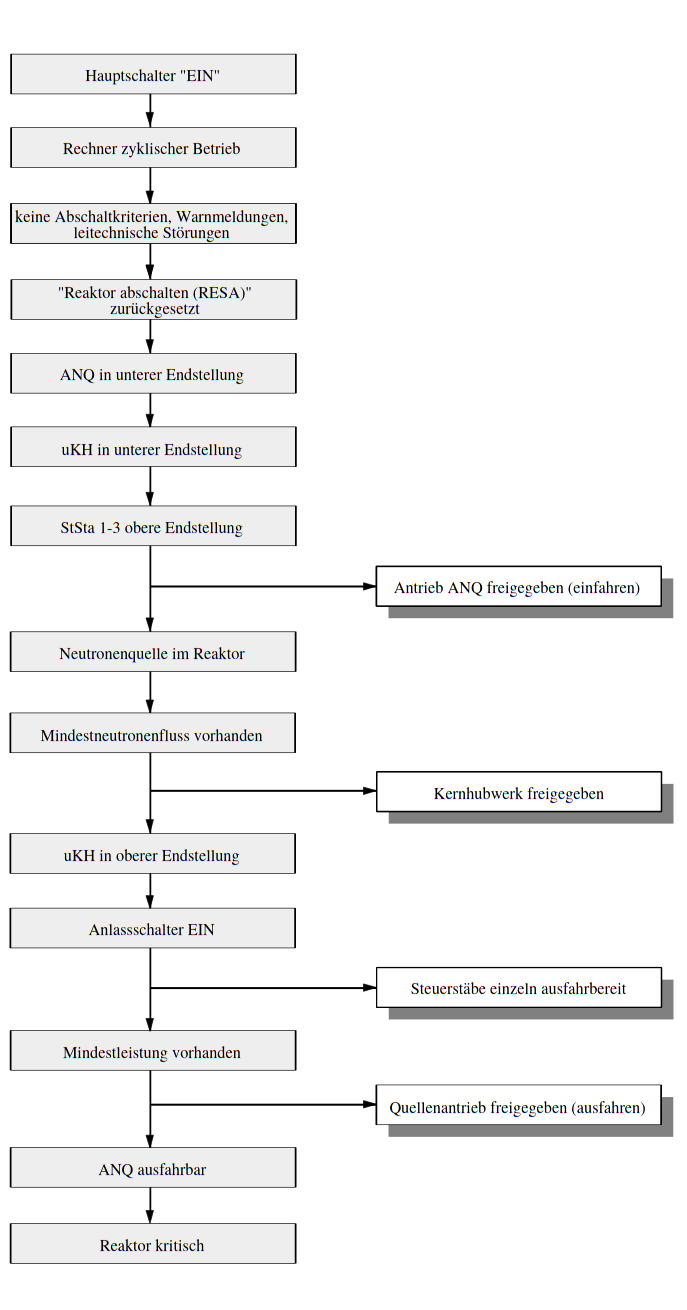
\includegraphics[width=0.7\textwidth]{/home/tom/GitHub_Repositories/Reaktor/Anlassschema.png}
\caption{Anfahrverriegelung, entnommen aus \cite{4}.}
\end{figure}


\newpage
Der Weg vom unterkritischen in den kritischen Zustand ist praktisch nicht durchführbar, da hierzu eine unendlich lange Wartezeit erforderlich wäre. Der kritische Zustand kann nur vom überkritischen Bereich aus erreicht werden.
Nachdem der Reaktor vom unterkritischen in den überkritischen Zustand versetzt wurde, nimmt seine Leistung gemäß Abb. 5 kontinuierlich zu. Der letzte Schritt besteht nun darin, den Reaktor bei der geforderten Leistung von exakt \(P=2.00\,\mathrm{W}\) kritisch zu machen. Dazu wartet man im überkritischen Betrieb ab, bis etwa \(80\,\%\) des Sollwertes erreicht sind und fährt dann die Steuerstäbe ein. Die Leistung nimmt dann weiter zu, allerdings wird die Verdopplungszeit immer länger. Somit kann man sich dem kritischen Zustand mit \(T=\infty\) von oben annähern und die geforderte Leistung erreichen. Für die Durchführung ist die Kenntnis des Reaktorverhaltens abhängig von seinem Zustand unerlässlich. Sie ist in Abb. 10 für die Leistung dargestellt: \\\\
\begin{figure}[h!]\centering
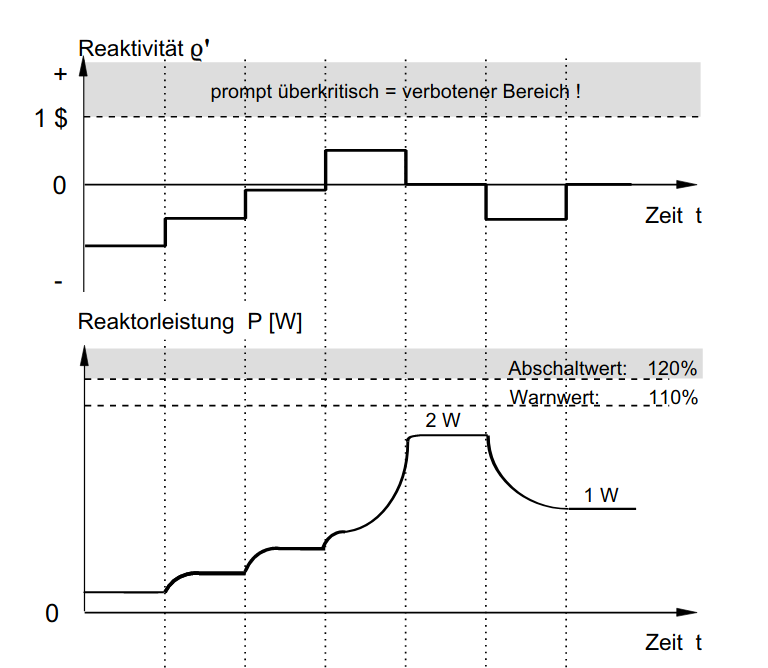
\includegraphics[width=0.8\textwidth]{Reaktion_des_Reaktors.png}
\caption{Reaktion der Reaktorleistung auf Änderungen der normierten Reaktivität, entnommen aus \cite{1}}
\end{figure}
\\\\
Die Reaktorleistung folgt prinzipiell der Reaktivitätsänderung hinsichtlich des Vorzeichens. Im unterkritischen Bereich gibt es dabei zunächst einen prompten Sprung und nach kurzer Zeit stellt sich ein konstanter Wert ein. Im überkritischen Bereich gibt es ebenfalls einen prompten Sprung. Es stellt sich jedoch kein konstanter Wert ein, sondern es kommt mit einer Verzögerung von etwa einer Minute zu einem exponentiellen Anwachsen der Leistung. Dieses für Reaktoren typische Verhalten wurde im Versuch beobachtet und ist wesentlich für die korrekte Steuerung von kerntechnischen Anlagen. Nach jedem Ein- oder Ausfahren der Steuerstäbe muss abgewartet werden, wie der Reaktor auf die veränderten Bedingungen reagiert. Insbesondere sind Messwerte der stabilen Reaktorperiode nur dann verlässlich und überhaupt sinnvoll, wenn die Zeitmessung erst nach erreichen des exponentiellen Anwachsens gestartet wurde. Die Einstellung der gewünschten Leistung ist damit auch mit einem gewissen zeitlichen Aufwand und Sorgfalt verbunden.
\subsection{Steuerstabkalibrierung}
    % Bibliographie/Literaturverzeichnis
    \begin{thebibliography}{9}
    \bibitem{1}
    Reaktorpraktikum. Versuch Reaktorstart. Versuchsanleitung. Technische Universität Dresden. Institut für Energietechnik.
    \bibitem{2}
    Reaktorpraktikum. Versuch Steuerstabkalibrierung. Versuchsanleitung. Technische Universität Dresden. Institut für           Energietechnik.
   \bibitem{3}
    Einführung Kernreaktorpraktikum. Technische Universität Dresden. Institut für           Energietechnik.
    \bibitem{4}
    Reaktorpraktikum. Beschreibung des Aufbaus, der Funktionskontrolle und der Betriebsprotokollierung. Technische Universität Dresden. Institut für Energietechnik.
    \bibitem{bindungsenergie}
    https://www.abiweb.de/physik-atomphysik-kernphysik/kernphysik-2/anwendung-nutzung-der-kernenergie.html (05.03.2020,      12:45)
  \bibitem{sigma_neutronen}
   https://www.wikiwand.com/de/Kernspaltung (05.03.2020, 13:02)
  \bibitem{spaltung_uran}
  https://www.4teachers.de/?action=keywordsearchsearchtype=imagessearchstring=Kernspaltung (05.03.2020, 13:26)
\bibitem{pe}
https://blog.ratioform.at/hdpe-ldpe-pp-pvc-und-was-sich-dahinter-verbirgt-eine-materialkunde/ (05.03.2020, 13:50)


    \end{thebibliography}

% Ende Dokument
\end{document}
